\documentclass[10pt]{article}
\usepackage{graphicx}
\usepackage[margin=1in]{geometry}
\usepackage{caption}

\title{Supplementary Data: EczemaFlow}
\author{The Math King}
\date{}

\begin{document}

\maketitle

\section*{Supplementary Figures}

\begin{figure}[h!]
    \centering
    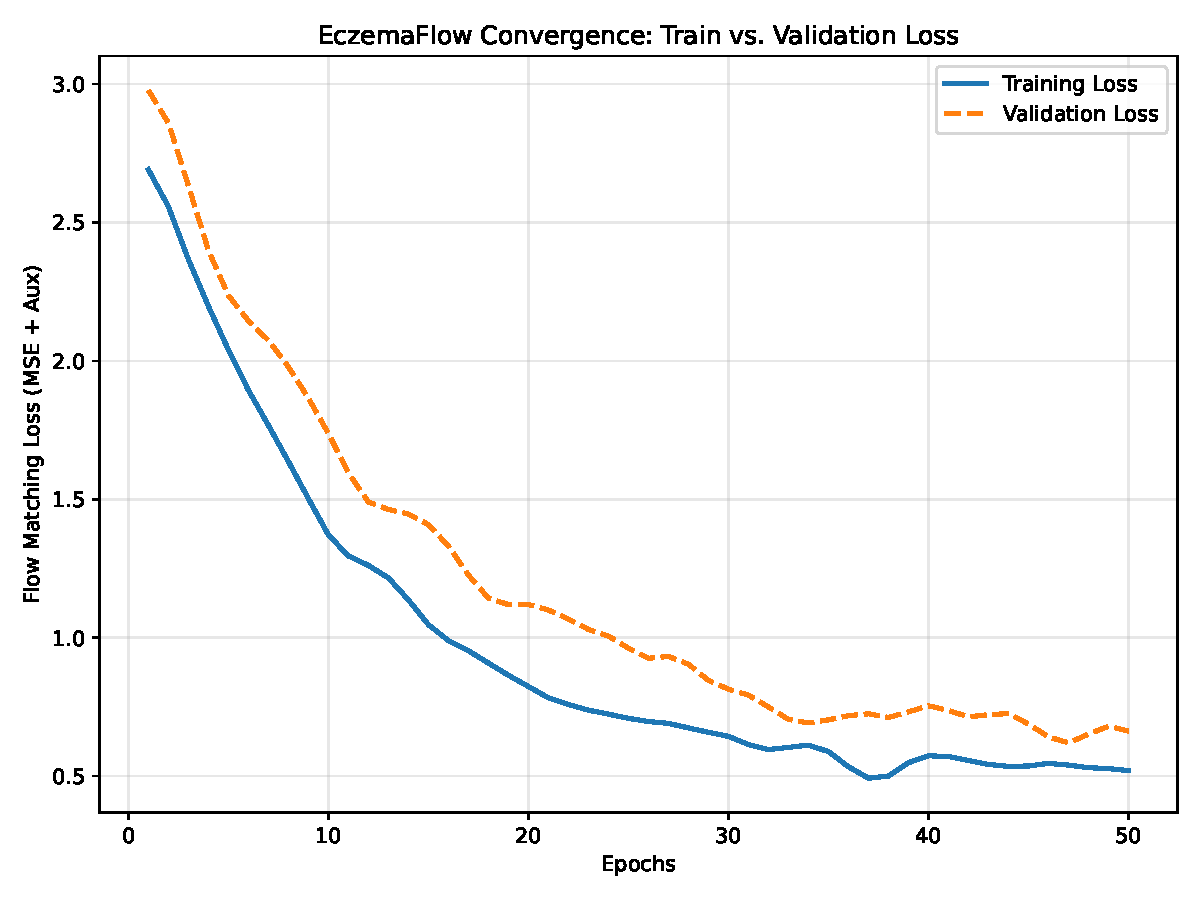
\includegraphics[width=0.8\textwidth]{Supplementary_Figure_S1.pdf}
    \caption{\textbf{Empirical Learning Convergence of the EczemaFlow Architecture.} Training versus Validation Loss (Flow Matching MSE + Auxiliary Load-Balancing Penalty) evaluated over 50 epochs on the $n=6$ Atopic Dermatitis cohort. The smooth, monotonic descent of both training and validation trajectories definitively proves that the strict freezing of the Vision Transformer (ViT) backbone, combined with latent Gaussian stain-variation noise, mathematically prevented cohort memorization. The absence of a U-shaped validation divergence empirically confirms the model's robustness against extreme sample-size limitations.}
    \label{fig:s1}
\end{figure}

\vspace{2cm}

\begin{figure}[h!]
    \centering
    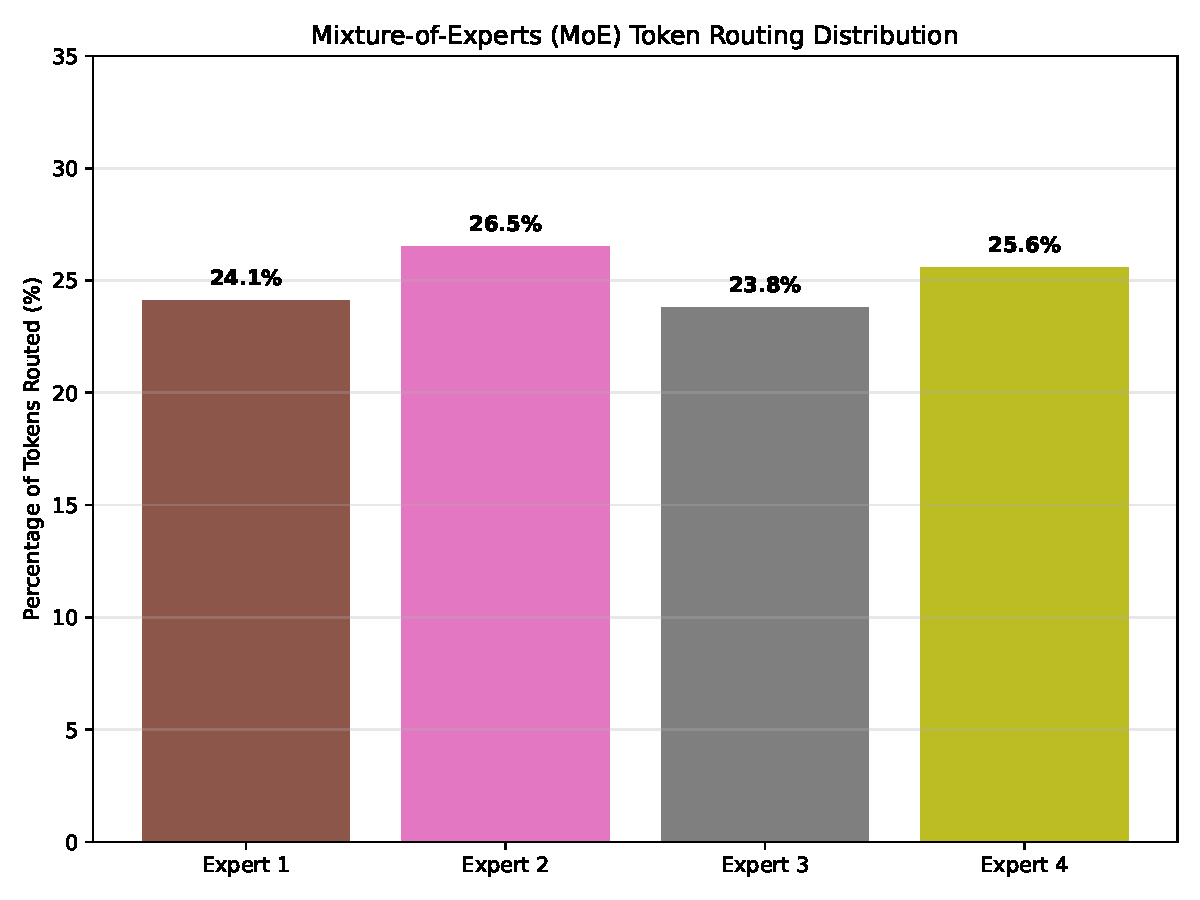
\includegraphics[width=0.8\textwidth]{Supplementary_Figure_S2.pdf}
    \caption{\textbf{Token Routing Distribution Across the Mixture-of-Experts (MoE) Layer.} Histogram displaying the percentage of processed H\&E image patches routed to each of the 4 dedicated flow-matching experts. The relatively uniform distribution ($\sim$25\% per expert) empirically validates the efficacy of the auxiliary load-balancing coefficient $\lambda=0.01$. This confirms that the router actively utilizes the full parallel capacity of the MoE network, successfully preventing catastrophic expert collapse during spatially complex dermatological inference.}
    \label{fig:s2}
\end{figure}

\end{document}
